% ============================================================
%  Chapter 3 — Method
% ============================================================
\chapter{Method}
\label{ch:method}

This chapter describes how our model works.
We start with the physical model that underlies IID (\secref{sec:physics}),
then describe the network architecture (\secref{sec:architecture}),
and finally explain the CARI training strategy (\secref{sec:cari}).


\section{Physical Model}
\label{sec:physics}

\subsection{The Standard IID Equation}

Under the Lambertian reflectance model with a single distant light source,
the intensity at a pixel $p$ in an image is:
\begin{equation}
  \mathbf{I}(p) = \mathbf{A}(p) \cdot S(p)
  \label{eq:iid}
\end{equation}
where $\mathbf{A}(p) \in [0,1]^3$ is the three-channel albedo (material
reflectance) and $S(p) \in \mathbb{R}_{>0}$ is a non-negative scalar shading
value. Shading describes the illumination arriving at the surface point after
geometry, visibility, and shadows have had their effect. Albedo describes the
fraction and colour of that light that the material diffusely reflects. The
camera observes the reflected result, not either factor in isolation.

Under the assumption of a grey (achromatic) illuminant, $S$ is a scalar and the
product in \eqnref{eq:iid} is a simple element-wise multiplication: each colour
channel of $\mathbf{I}$ is scaled by the same amount.
This makes the colour of each pixel determined entirely by $\mathbf{A}$.

\subsection{Why Achromatic Shading Fails with Coloured Light}

When the illuminant has colour, the scaling is no longer the same across channels.
A red lamp makes the $R$ channel brighter relative to $G$ and $B$.
A correct model would encode this in the shading, but scalar shading cannot express
different scalings per channel.
What actually happens in practice is that the model absorbs the channel imbalance
into the albedo, because the albedo is the only RGB term in the equation.
The predicted albedo therefore reflects the combined colour of the surface
\emph{and} the illuminant, rather than just the surface.

\figref{fig:formulation} demonstrates that this is a limitation of the
representation, not a particular network. Even when the scalar model is given
the luminance of the true RGB shading, dividing the image by that scalar can
change brightness but cannot remove the lamp's hue.

\begin{figure}[t!]
  \centering
  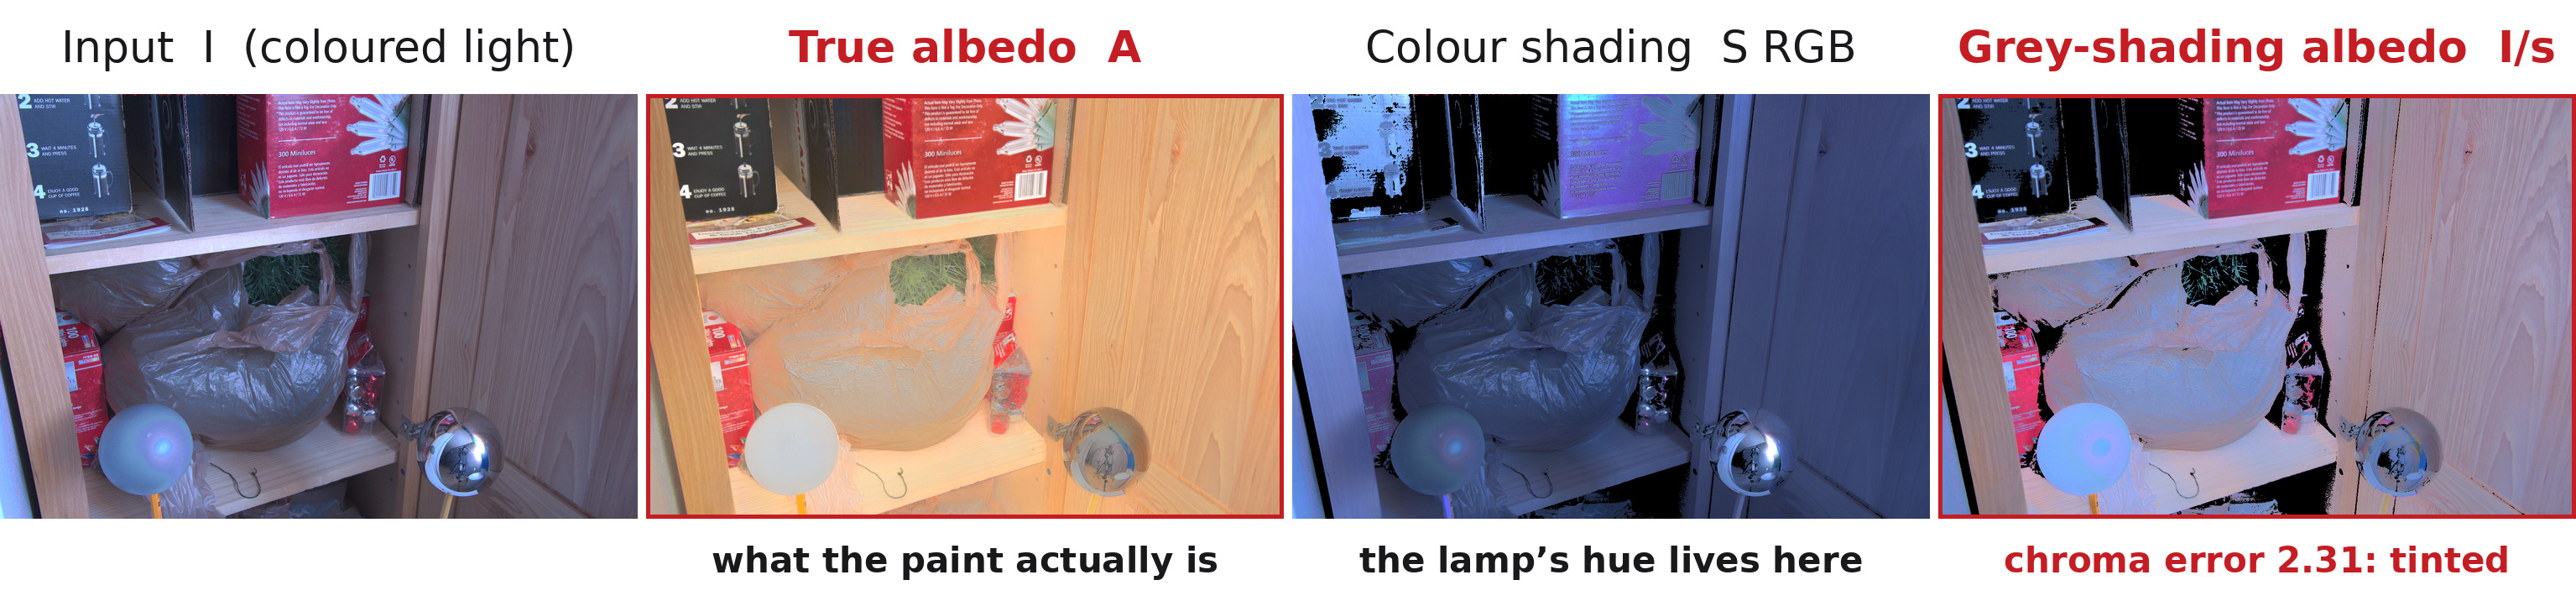
\includegraphics[width=\textwidth]{images/formulation/formulation.jpg}
  \caption[Why scalar shading leaks illuminant colour into albedo.]{%
    Why scalar shading must leak illuminant colour into albedo. From left: a
    warm-lit MID frame; pseudo-ground-truth albedo; the RGB shading implied by
    the data; and the albedo recovered with the luminance of that true shading.
    The favourable scalar construction still produces a
    visibly tinted albedo (mean chroma error $2.31$, versus $0.22$ when shading
    has three channels), because a scalar can alter brightness but not hue. The
    remaining RGB error comes from clipping and the display-domain conversion,
    not from an inability to represent channel-dependent illumination.
  }
  \label{fig:formulation}
\end{figure}

To model coloured illumination correctly, the shading must therefore be a
three-channel (RGB) quantity $\mathbf{S}_d(p) \in \mathbb{R}_{>0}^3$, so each
colour channel can be scaled independently.
The model additionally keeps an explicit non-diffuse term for the light that the
Lambertian product cannot represent (specular highlights, visible light sources,
clipped pixels), giving the full decomposition:
\begin{equation}
  \mathbf{I}(p) = \mathbf{A}(p) \odot \mathbf{S}_d(p) + \mathbf{R}(p)
  \label{eq:iid_color}
\end{equation}
where $\odot$ is element-wise multiplication, $\mathbf{S}_d$ is the colored
\emph{diffuse} shading, and $\mathbf{R} \geq 0$ is the non-diffuse residual.
The model predicts $\mathbf{A}$ and $\mathbf{S}_d$ with two network heads and derives
the residual \emph{analytically} as
$\mathbf{R} = \bigl(\mathbf{I} - \mathbf{A} \odot \mathbf{S}_d\bigr)_{+}$,
so the reconstruction $\mathbf{A} \odot \mathbf{S}_d + \mathbf{R}$ matches the
input by construction wherever the diffuse product does not overshoot it.

A three-channel shading solves the representation problem but not the
\emph{ambiguity} problem: single-image supervision cannot say how much of a hue
belongs to the albedo and how much to the shading colour, and the standard
ground-truth datasets (including Hypersim) supervise shading only up to this
ambiguity.
This is where CARI comes in: by constraining the albedo to be identical across
images of the same scene under different illuminants, the colour split stops
being a free choice: any illuminant colour that the model puts into the albedo
now violates the invariance constraint, so it is forced into $\mathbf{S}_d$,
which is exactly where the physics says it belongs.

\subsection{The Shading Parameterisation}

A practical challenge in predicting shading is that it can take any positive
value, which is an unbounded output range; worse, its distribution in
real scenes is heavily skewed.
Specular surfaces and bright light sources produce very large shading values,
so linear shading concentrates almost all pixels in a narrow band near zero
with a long tail (\figref{fig:inverse_shading}): a regression loss on this
representation is dominated by a few extreme pixels while the mid-range
values that carry the shadow structure receive almost no gradient.
Working in the logarithmic domain balances the distribution but still has no
well-defined range for a network output.
Following the inverse-shading parameterisation of \mycitetext{careaga23ordinal},
which was introduced to solve exactly this conditioning problem,
the network predicts a bounded quantity
$\boldsymbol{\pi}(p) = 1 / \bigl(\mathbf{S}_d(p) + 1\bigr) \in (0, 1)$
per channel using a sigmoid activation, and the shading is recovered by
inverting this mapping:
\begin{equation}
  \mathbf{S}_d(p) = \frac{1 - \boldsymbol{\pi}(p)}{\boldsymbol{\pi}(p)}
  \label{eq:uninvert}
\end{equation}
The prediction is clamped to
$\boldsymbol{\pi} \in [5 \times 10^{-3},\, 1 - 10^{-4}]$, which bounds the
recovered shading to $\mathbf{S}_d \in [10^{-4},\, 199]$, providing enough headroom to
represent bright high-dynamic-range illumination while keeping the division
numerically safe.
The inversion is differentiable, so gradients flow through it during training.
Losses that supervise the shading pattern are computed on $\boldsymbol{\pi}$
(bounded, well-conditioned), while physics losses that need the actual light
intensity (reconstruction, the residual) use the linear $\mathbf{S}_d$.

% fig:inverse_shading — regenerated from our own Hypersim data by
% tests/viz/build_inverse_shading_figure.py. The panels are raster (they are images); the
% three distributions are drawn here as pgfplots so they are vector, sharp at any zoom, and
% set in the document's own fonts. Data: chapters/data/shading_hist_*.dat
\begin{figure}[t!]
  \centering
  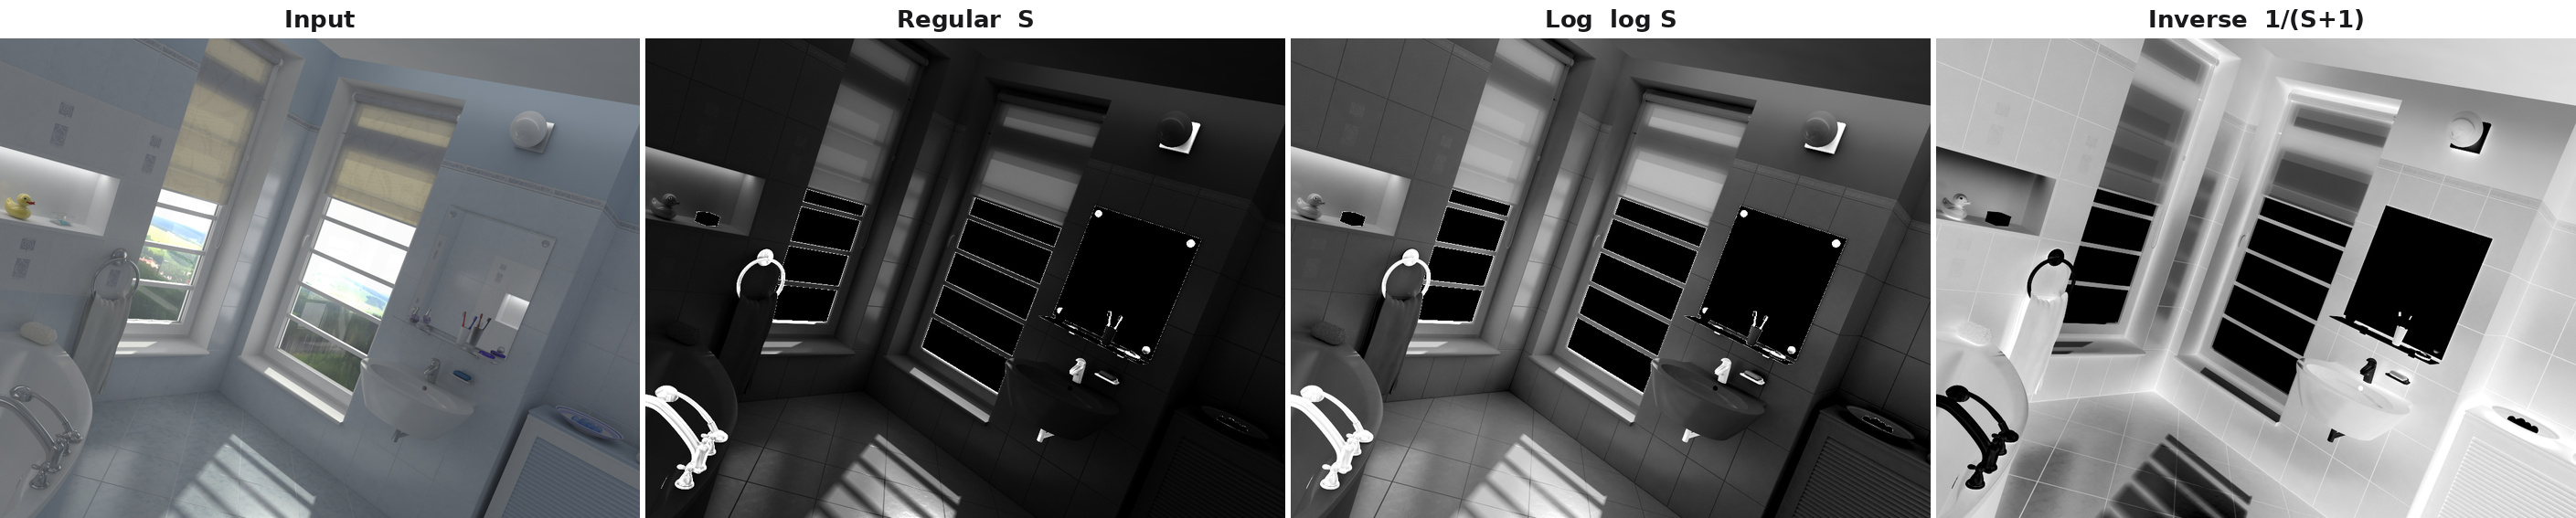
\includegraphics[width=\textwidth]{images/inverse_shading/panels.jpg}\\[6pt]
  \pgfplotsset{
    shadinghist/.style={
      width=0.35\textwidth, height=3.6cm,
      ybar, bar width=1.1pt,
      ymin=0, ymax=1.10,
      axis lines=left,
      axis line style={gray!55},
      tick label style={font=\scriptsize},
      xlabel style={font=\scriptsize, yshift=2pt},
      ylabel style={font=\scriptsize},
      ytick=\empty,
      minor tick num=0,
      xtick align=outside,
      grid=none,
      title style={font=\scriptsize, yshift=-2pt},
      every axis plot/.append style={
        fill=blue!50!cyan, draw=none},
    }}
  \begin{tikzpicture}
    \begin{axis}[shadinghist, xlabel={$S$ \, (linear)}, ylabel={density},
                 xmin=-0.15, xmax=5.4, xtick={0,1,2,3,4,5},
                 title={Regular: mass collapses at $0$}]
      \addplot table[x=x, y=y] {chapters/data/shading_hist_regular.dat};
    \end{axis}
  \end{tikzpicture}\hfill
  \begin{tikzpicture}
    \begin{axis}[shadinghist, xlabel={$\log S$},
                 xmin=-1.75, xmax=1.8, xtick={-1.5,-0.5,0.5,1.5},
                 title={Log: balanced but unbounded}]
      \addplot table[x=x, y=y] {chapters/data/shading_hist_log.dat};
    \end{axis}
  \end{tikzpicture}\hfill
  \begin{tikzpicture}
    \begin{axis}[shadinghist, xlabel={$1/(S+1)$},
                 xmin=-0.03, xmax=1.03, xtick={0,0.25,0.5,0.75,1},
                 title={Inverse: spread across $[0,1]$}]
      \addplot table[x=x, y=y] {chapters/data/shading_hist_inverse.dat};
    \end{axis}
  \end{tikzpicture}
  \caption[Inverse-shading parameterisation and target distributions.]{%
    Why shading is regressed in the inverse domain. Shading is derived from Hypersim ground
    truth as $S = \mathbf{I} / \mathbf{A}$ and shown in three representations, with the
    distribution of its values beneath each.
    Linear shading is dominated by a small number of very bright pixels. It runs to
    $5.3$ on this frame, so almost all of the mass collapses into the first bin and a
    regressor spends its capacity on outliers.
    Log shading balances the distribution but has no bounded range, so it cannot be produced
    by a saturating output nonlinearity.
    Inverse shading, $1/(S+1)$, is confined to $[0,1]$ \emph{by construction} and spreads
    across it, which makes it a well-conditioned target for a sigmoid head: this is the
    representation our shading branch predicts (\secref{sec:physics}), following
    \mycitetext{careaga23ordinal}. The physics losses that need real light intensity operate
    on the linear $\mathbf{S}_d$ recovered from it.
  }
  \label{fig:inverse_shading}
\end{figure}



\section{Network Architecture}
\label{sec:architecture}

Our model is built on two components: a frozen DINOv2-Large visual encoder and a
DPT-style decoder with separate output heads for albedo and shading.

\subsection{DINOv2 Encoder}

The encoder is DINOv2-Large \mycite{oquab24dinov2}, a Vision Transformer (ViT)
with a patch size of 14 pixels and approximately 304 million parameters.
DINOv2 was trained with self-supervised learning on a large and diverse image
corpus, and it produces patch-level feature representations that capture
rich semantic and geometric information.

We use DINOv2 in a frozen state, meaning its weights are not updated during
IID training.
This is a deliberate design choice for two reasons.
First, DINOv2's representations are already very strong; fine-tuning them would
require careful learning rate scheduling and risks destroying useful features
learned during self-supervised pre-training.
Second, keeping the encoder frozen reduces GPU memory during training, which
allows us to use a larger batch size.

For an input image of size $H \times W$, DINOv2 divides it into $(H/14) \times (W/14)$
patches and produces a token embedding for each patch.
We extract the intermediate features from four roughly evenly-spaced transformer
blocks (blocks 5, 12, 18, and 24 of the 24-block ViT-L, the last of which is the
final block).
These multi-depth features capture information at different levels of abstraction:
earlier blocks retain more local texture and colour, while later blocks encode
semantic and structural information.
One consequence of DINOv2's heavily augmented self-supervised training is
directly useful for IID: because its objective is invariant to strong
photometric augmentation, its patch tokens are expected to be robust to
low-level appearance changes including illumination, so a shadowed and a lit
patch of the same material tend to map to similar tokens, which is a helpful prior for
assigning the same albedo across a shadow boundary.

\subsection{DPT Decoder}

The Dense Prediction Transformer (DPT) decoder \mycite{ranftl21dpt} was designed
to reconstruct full-resolution feature maps from the patch tokens of a ViT.
The key idea is to re-assemble the patch tokens from each layer into a spatial
feature map, then fuse the maps from all layers through a series of convolutional
feature fusion blocks.
The fusion progressively upsamples the features to the input resolution,
combining coarse semantic information from deep layers with fine spatial details
from early layers.

We use a single DPT decoder that takes all four feature levels as input.
Each level is first \emph{reassembled}: the patch tokens are projected and
reshaped into a spatial feature map at a level-specific resolution.
The four maps are then merged by a chain of \emph{fusion} blocks, each of
which upsamples the coarser map, adds the next finer one, and refines the sum
with residual convolutions, so semantic context from deep blocks and spatial
precision from early blocks accumulate into one representation.
Because the ViT operates on $14 \times 14$ patches, even the finest token map
is far below pixel resolution; a lightweight convolutional \emph{detail stem}
therefore processes the raw input image in parallel and injects genuine
high-frequency edge information that the token path cannot carry.
The decoder output is a shared full-resolution feature map, which is fed to
two separate output heads.

\subsection{Output Heads}

The albedo head takes the DPT feature map, concatenates a full-resolution
\emph{RGB skip} (the gamma-encoded input image), and passes the result through
a small convolutional block followed by a sigmoid activation:
\begin{equation}
  \mathbf{A} = \sigma\Bigl(\text{Conv}\bigl(\mathbf{F}_{\text{DPT}},\,
               \mathbf{I}^{1/2.2}\bigr)\Bigr) \in [0, 1]^{H \times W \times 3}
  \label{eq:albedo_head}
\end{equation}
The sigmoid bounds the albedo to $[0,1]^3$, the correct range for a reflectance
value.
The RGB skip is motivated by a practical risk of using a frozen semantic encoder:
its tokens need not retain all of the local, absolute colour information required
for albedo prediction. We did not directly probe DINOv2 for illumination
invariance, so this is a design hypothesis rather than an established property of
the encoder. Feeding image colour directly into the head restores that capacity.
Crucially, this skip is only safe \emph{in combination with} the CARI invariance
loss: with a direct colour path and no invariance constraint, the illuminant
colour would flow straight through the skip into the albedo.
This coupling is one of the ablation axes in \chapref{ch:experiments}.

The shading head applies its own convolutional block and sigmoid and outputs the
three-channel inverse shading:
\begin{equation}
  \boldsymbol{\pi} = \sigma\bigl(\text{Conv}(\mathbf{F}_{\text{DPT}})\bigr)
  \in (0, 1)^{H \times W \times 3}
  \label{eq:shading_head}
\end{equation}
The colored diffuse shading $\mathbf{S}_d$ is recovered from $\boldsymbol{\pi}$
using \eqnref{eq:uninvert}, and the non-diffuse residual follows analytically:
\begin{equation}
  \mathbf{R} = \bigl(\mathbf{I} - \mathbf{A} \odot \mathbf{S}_d\bigr)_{+}
  \label{eq:residual}
\end{equation}
There is no third head: the residual costs no parameters, and the reconstruction
$\mathbf{A} \odot \mathbf{S}_d + \mathbf{R}$ is exact wherever the diffuse
product does not overshoot the image.

Both heads share the same DPT feature map as input.
This encourages the two predictions to be consistent with each other, since they
are both derived from the same underlying scene representation.

% fig:architecture — CRefNet-style pipeline for our model, with the supervised losses.
% Thumbnails: tests/viz/gen_arch_thumbs.py (data-only model), images/arch/*.png.
\begin{figure}[p]
  \centering
  \resizebox{\textwidth}{!}{%
  \begin{tikzpicture}[
      font=\sffamily, >=latex,
      thumb/.style={inner sep=0pt, draw=black!55, line width=0.4pt},
      blk/.style={draw=black!45, rounded corners=2pt, align=center, minimum height=15mm,
                  minimum width=12mm, line width=0.5pt, font=\small},
      dino/.style={blk, fill=teal!16, draw=teal!55, minimum height=30mm},
      dpt/.style={blk, fill=myblue!14, draw=myblue!55, minimum height=30mm},
      head/.style={blk, fill=orange!16, draw=orange!60},
      resid/.style={blk, fill=black!12, draw=black!50, minimum width=30mm},
      loss/.style={draw=red!55!black, circle, fill=red!7, inner sep=1pt, minimum size=8.5mm,
                   font=\footnotesize, text=red!60!black},
      io/.style={align=center, font=\small},
      dim/.style={font=\scriptsize\itshape, text=black!55, align=center},
      flow/.style={->, line width=0.8pt, black!70},
      lossflow/.style={->, line width=0.6pt, red!55!black},
      skipC/.style={->, line width=0.9pt, red!62!black, dashed},
      skipL/.style={->, line width=0.9pt, black!55, dash pattern=on 3pt off 2pt},
    ]
    % rows: albedo (top, y=+11), trunk (mid, y=0), shading (bottom, y=-11)
    % ── encoder + decoder (mid row) ─────────────────────────────────
    \node[thumb] (imgT) at (0,0) {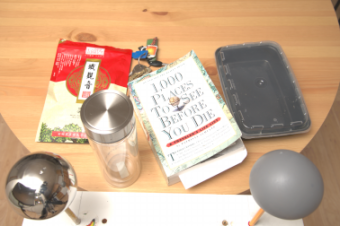
\includegraphics[width=19mm]{images/arch/input.png}};
    \node[io, above=0.5mm of imgT] {Input $\mathbf{I}$};
    \node[dino, right=9mm of imgT] (dino) {DINOv2-L/14\\[2pt]\emph{frozen}\\[2pt]{\scriptsize 4 stages, $\mathrm{d}{=}1024$}};
    \node[dim, above=0.4mm of dino] {material tokens};
    \node[dpt, right=10mm of dino] (dpt) {DPT\\decoder};
    \node[dim, below=0.5mm of dpt] {$768{\to}384{\to}192{\to}96{\to}64$};

    % ── heads (top / bottom rows) ───────────────────────────────────
    \node[head, above right=7mm and 12mm of dpt] (ah) {Albedo\\head};
    \node[head, below right=7mm and 12mm of dpt] (sh) {Shading\\head};

    % ── outputs + thumbnails ────────────────────────────────────────
    \node[io, right=8mm of ah] (Asym) {$\mathbf{A}\!\in\![0,1]^3$};
    \node[thumb, right=2.5mm of Asym] (albT) {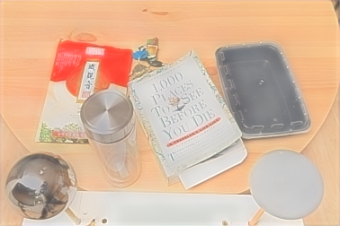
\includegraphics[width=15mm]{images/arch/albedo.png}};
    \node[io, right=8mm of sh] (Ssym) {$\boldsymbol{\pi}\!\in\!(0,1)^3$\\[1pt]$\mathbf{S}_d{=}\tfrac{1-\boldsymbol{\pi}}{\boldsymbol{\pi}}$};
    \node[thumb, right=2.5mm of Ssym] (shaT) {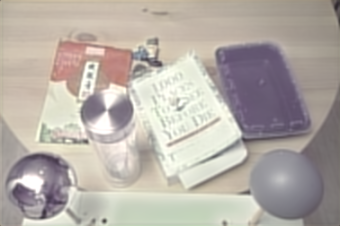
\includegraphics[width=15mm]{images/arch/shading.png}};

    % ── analytic residual: MUST sit downstream (right) of albT/shaT, since it is
    % computed FROM A and S_d. Placing it to their left (as an earlier draft did) forces
    % the A-> R and S_d->R arrows to run right-to-left, against the diagram's own
    % left-to-right reading order — that was the misleading part. Anchored off albT/shaT
    % themselves (not off dpt) so it automatically stays downstream of them.
    % Pin R's height EXACTLY to dpt/imgT's row (the guessed yshift offset in an earlier
    % draft was wrong). imgT, dino and dpt are chained with plain "right=" (no vertical
    % component), so they share one y; extracting x from albT.east and y from dpt.center
    % directly, via `let`, removes any guesswork about node-anchor offsets.
    \path let \p1 = ([xshift=20mm]albT.east), \p2 = (dpt.center) in
      node[resid] (R) at (\x1,\y2)
      {$\mathbf{R}{=}(\mathbf{I}{-}\mathbf{A}{\odot}\mathbf{S}_d)_{+}$\\[1pt]{\scriptsize analytic; \emph{no head}}};
    % Residual thumbnail sits to R's RIGHT (not below), on the way to its loss, mirroring
    % how albT/shaT sit between their heads and their own loss nodes.
    \node[thumb, right=6mm of R] (resT) {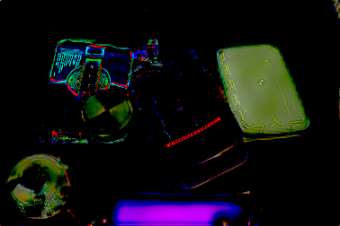
\includegraphics[width=13mm]{images/arch/residual.png}};

    % ── flows ───────────────────────────────────────────────────────
    \draw[flow] (imgT) -- (dino);
    \draw[flow] (dino) -- node[dim,above]{4 lvls} (dpt);
    \draw[flow] (dpt.east) -- ++(3mm,0) |- (ah.west);
    \draw[flow] (dpt.east) -- ++(3mm,0) |- (sh.west);
    \draw[flow] (ah) -- (Asym); \draw[flow] (Asym) -- (albT);
    \draw[flow] (sh) -- (Ssym); \draw[flow] (Ssym) -- (shaT);
    % A and S_d both feed R from the LEFT (upstream), arrowheads pointing right/down and
    % right/up INTO R — matches the left-to-right flow of the rest of the diagram.
    \draw[flow] (albT.south) -- ++(0,-4mm) -| (R.north);
    \draw[flow] (shaT.north) -- ++(0,4mm)  -| (R.south);

    % ── physics-typed skips ─────────────────────────────────────────
    \draw[skipC] (imgT.north) |- ([yshift=7mm]ah.north) -| (ah.north)
      node[dim,pos=0.25,above,text=red!55!black]{RGB skip $\mathbf{I}^{1/2.2}$ (3\,ch, colour)};
    \draw[skipL] (imgT.south) |- ([yshift=-7mm]sh.south) -| (sh.south)
      node[dim,pos=0.25,below]{luminance skip (1\,ch, intensity)};

    % ── SUPERVISED LOSSES (right column) ────────────────────────────
    \node[loss, right=10mm of albT] (la) {$\mathcal{L}_{\text{a}}$};
    \node[dim, right=0.5mm of la, text=red!55!black, align=left]
      {$+\,\mathcal{L}_{\text{msg-a}},\mathcal{L}_{\text{dssim}}$\\$+\,\mathcal{L}_{\text{chroma}},\mathcal{L}_{\text{mat}}$};
    \node[loss, right=10mm of shaT] (ls) {$\mathcal{L}_{\text{s}}$};
    \node[dim, right=0.5mm of ls, text=red!55!black, align=left]
      {$+\,\mathcal{L}_{\text{msg-s}},\mathcal{L}_{\text{sign}}$};
    % R.north = incoming A, R.south = incoming S_d (set above); R.east feeds the residual
    % thumbnail, which in turn feeds L_res — the same pattern albT->la and shaT->ls use.
    \node[loss, right=8mm of resT] (lr) {$\mathcal{L}_{\text{res}}$};
    \node[dim, above=0.3mm of lr, text=red!55!black]{sparsity $|\mathbf{R}|{\to}0$};

    \draw[lossflow] (albT) -- (la);
    \draw[lossflow] (shaT) -- (ls);
    \draw[flow] (R.east) -- (resT.west);
    \draw[lossflow] (resT.east) -- (lr);
    % CARI acts on the albedo too (training-only; detailed in fig:cari)
    \node[loss, above=4mm of la, draw=red!55!black, fill=red!7] (linv) {$\mathcal{L}_{\text{inv}}$};
    \node[dim, right=0.5mm of linv, text=red!55!black, align=left]{cross-render\\(\figref{fig:cari})};
    \draw[lossflow, dashed] (albT.north) to[bend left=12] (linv.west);

    % ── legend (own row, below everything) ──────────────────────────
    \coordinate (legY) at ([yshift=-24mm]sh.south -| imgT.west);
    \begin{scope}[shift={(legY)}]
      \node[dino, minimum height=5mm, minimum width=7mm] (l1) {};
      \node[io, right=1.5mm of l1] (l1t){frozen encoder};
      \node[dpt, minimum height=5mm, minimum width=7mm, right=7mm of l1t] (l2) {};
      \node[io, right=1.5mm of l2] (l2t){DPT decoder \scriptsize(trained)};
      \node[head, minimum height=5mm, minimum width=7mm, right=7mm of l2t] (l3) {};
      \node[io, right=1.5mm of l3] (l3t){output head \scriptsize(trained)};
      \node[loss, minimum size=6mm, right=8mm of l3t] (l4) {};
      \node[io, right=1.5mm of l4] (l4t){loss};
      \draw[skipC] ([xshift=8mm]l4t.east) -- ++(6mm,0);
      \node[io, right=1mm of l4t, xshift=14mm] (sc){colour skip};
      \draw[skipL] ([xshift=7mm]sc.east) -- ++(6mm,0);
      \node[io, right=13mm of sc]{intensity skip};
    \end{scope}
  \end{tikzpicture}}
  \caption[Model architecture and supervision.]{%
    Model architecture and its supervision. A \emph{frozen} DINOv2-Large encoder (teal)
    extracts patch features from four transformer stages; because it is never fine-tuned it
    supplies the illumination-invariant material tokens the backbone was pre-trained to
    produce, and only $18.5$M parameters downstream are learned. A DPT decoder (blue)
    reassembles and fuses the four levels into a shared full-resolution feature map. Two
    output heads (amber) read it, each with a \emph{physics-typed} full-resolution skip from
    the input: the albedo head takes the gamma-encoded RGB image (a colour path) and predicts
    $\mathbf{A}$; the shading head takes only the input luminance (an intensity path) and
    predicts the inverse shading $\boldsymbol{\pi}$, from which
    $\mathbf{S}_d=(1-\boldsymbol{\pi})/\boldsymbol{\pi}$ follows. The non-diffuse residual
    $\mathbf{R}=(\mathbf{I}-\mathbf{A}\odot\mathbf{S}_d)_{+}$ is analytic; there is no third
    head. Red nodes are the training losses on each output: the albedo family
    ($\mathcal{L}_{\text{a}}$ with its multi-scale-gradient, structural, chroma and
    material-consistency terms), the shading family ($\mathcal{L}_{\text{s}}$ with its
    gradient and sign terms), and a sparsity term $\mathcal{L}_{\text{res}}$ that pushes the
    analytic residual toward zero. The cross-render invariance loss $\mathcal{L}_{\text{inv}}$
    also constrains the albedo but acts across an illuminant pair at training time only
    (\figref{fig:cari}). Thumbnails are this model's own outputs on a MID test scene.
  }
  \label{fig:architecture}
\end{figure}



\section{Cross-Render Albedo Invariance (CARI)}
\label{sec:cari}

\subsection{The Core Idea}

CARI is a training strategy, not a change to the network.
It adds two loss terms that operate on \emph{pairs} of images of the same scene
photographed under different illuminants.

Let $(\mathbf{I}_1, \mathbf{I}_2)$ be such a pair, where $\mathbf{I}_1$ and
$\mathbf{I}_2$ show the same scene under two different coloured light sources.
Let $\mathbf{A}_1 = \mathbf{A}(\mathbf{I}_1)$ and $\mathbf{A}_2 = \mathbf{A}(\mathbf{I}_2)$
be the albedos predicted by the model for each image, and let $S_1$ and $S_2$ be
the corresponding shadings.

\subsection{Invariance Loss}

The albedo must be the same for both images, because the physical material has not
changed.
We encode this as a masked $\ell_1$ loss:
\begin{equation}
  \mathcal{L}_{\text{inv}} =
  \frac{1}{|\Omega_v|} \sum_{p \in \Omega_v}
  \bigl\| \mathbf{A}_1(p) - \mathbf{A}_2(p) \bigr\|_1
  \label{eq:linv}
\end{equation}
where $\Omega_v \subset \Omega$ is the set of \emph{valid paired pixels}.
The validity mask matters in practice: MID frames are high-dynamic-range captures
that are clipped per frame, so a pixel can be saturated in one frame and not the
other, and deep shadows carry mostly sensor noise.
$\Omega_v$ excludes clipped and near-black pixels in either frame (roughly 75\%
of pixels survive the mask on average), so the invariance constraint is only
applied where both observations are trustworthy.
This loss is zero only when the model predicts identical albedo for both images.
Minimising it forces the model to make the albedo independent of the illuminant
colour.

\subsection{Explanation Loss}

The invariance loss alone is not enough.
A degenerate model could satisfy \eqnref{eq:linv} by predicting a flat, constant
albedo (the same grey image for every input).
To prevent this, we add a companion loss that requires the shading to \emph{explain}
the pixel-level difference between the two images.

Under the diffuse model $\mathbf{I} \approx \mathbf{A} \odot \mathbf{S}_d$, the
ratio of corresponding pixels in the two images equals the ratio of their
shadings wherever the albedo is shared:
\begin{equation}
  \frac{\mathbf{I}_1(p)}{\mathbf{I}_2(p)} = \frac{\mathbf{S}_{d,1}(p)}{\mathbf{S}_{d,2}(p)},
  \qquad \text{if } \mathbf{A}_1(p) = \mathbf{A}_2(p)
  \label{eq:explain_ratio}
\end{equation}
The material term cancels in the ideal diffuse image ratio, making the ratio a
useful lighting cue wherever registration is valid and non-diffuse effects are
small. Saturation, shadows, and specularities violate that idealisation; the
validity mask limits rather than eliminates those failures.
We enforce the constraint on the \emph{luminance} of both ratios, in the log
domain for numerical robustness:
\begin{equation}
  \mathcal{L}_{\text{expl}} =
  \frac{1}{|\Omega_v|} \sum_{p \in \Omega_v}
  \Bigl|
    \log\frac{L(\mathbf{I}_1(p)) + \varepsilon}{L(\mathbf{I}_2(p)) + \varepsilon}
  - \log\frac{L(\mathbf{S}_{d,1}(p)) + \varepsilon}{L(\mathbf{S}_{d,2}(p)) + \varepsilon}
  \Bigr|
  \label{eq:lexpl}
\end{equation}
where $L(\cdot)$ is the Rec.~601 luminance, $\varepsilon = 10^{-3}$, and
$\Omega_v$ is the same validity mask as in \eqnref{eq:linv}.
Using luminance makes this term supervise the achromatic \emph{intensity} change
between the frames. Colour separation is produced by the interaction of the
three-channel decomposition, albedo/reconstruction supervision, and
$\mathcal{L}_{\text{inv}}$; the invariance term alone does not identify where the
rejected colour must go.
This loss is zero only when the shading ratio matches the image ratio at every
valid pixel, which means the shading is absorbing the lighting difference rather
than the albedo.

\subsection{Why Raw (Un-White-Balanced) Pairs Are Necessary}
\label{sec:raw_pairs}

A subtle but important point about applying CARI is the role of white balance.
Standard image pre-processing in most datasets applies automatic white balance,
which estimates the illuminant and rescales the colour channels so that neutral
surfaces appear neutral. A common heuristic is the \emph{grey-world} assumption:
the average scene reflectance is treated as grey. It fails when the scene itself
is not colour-balanced. For example, in a room dominated by a red painted wall,
the average red signal can come from the material rather than the lamp; forcing
that average to grey removes genuine wall colour. White balance is therefore an
estimate, not ground truth.
After white balance, the two images $\mathbf{I}_1$ and $\mathbf{I}_2$ of the same
scene under different illuminants will look very similar in terms of global colour,
because the illuminant colour has been removed.

This is precisely the wrong input for CARI.
The luminance explanation loss in \eqnref{eq:lexpl} needs the intensity change,
whereas the colour variation is needed by the RGB invariance and reconstruction
constraints. If both images are white-balanced to look neutral, much of that RGB
variation is removed before training, so CARI can no longer teach the model which
colour belongs to the illuminant rather than the surface.

We confirm this by measuring the chromaticity spread of the MID dataset with and
without white balance.
The ground-truth illuminant probes show 15--25\% variation in chromaticity across
the different illuminant conditions; this variation is almost entirely removed by
white balance.
We therefore set the \texttt{mid\_raw\_color\_pair} flag to \texttt{true} in our
training configuration, which disables white balance for MID pairs.

% fig:cari — CARI training diagram, styled to match fig:architecture.
% Thumbnails from tests/viz/gen_cari_thumbs.py (documents/thesis/images/arch/cari_*.png).
\begin{figure}[t!]
  \centering
  \resizebox{0.96\textwidth}{!}{%
  \begin{tikzpicture}[
      font=\sffamily, >=latex,
      thumb/.style={inner sep=0pt, draw=black!55, line width=0.4pt},
      model/.style={draw=myblue!55, fill=myblue!12, rounded corners=2pt, align=center,
                    minimum width=17mm, minimum height=34mm, line width=0.5pt},
      loss/.style={draw=red!55!black, circle, fill=red!7, inner sep=1pt, minimum size=11mm,
                   font=\small, text=red!60!black},
      io/.style={align=center, font=\small},
      dim/.style={font=\scriptsize\itshape, text=black!55, align=center},
      flow/.style={->, line width=0.8pt, black!70},
    ]

    % ── the cross-illuminant input pair (real, pixel-aligned) ───────
    \node[thumb] (i1) {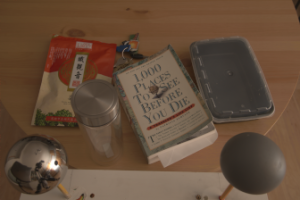
\includegraphics[width=20mm]{images/arch/cari_I1.png}};
    \node[io, above=0.5mm of i1] {$\mathbf{I}_1$ \scriptsize(warm light)};
    \node[thumb, below=12mm of i1] (i2) {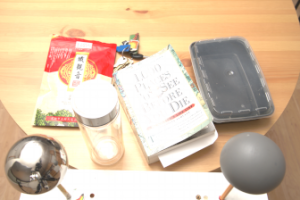
\includegraphics[width=20mm]{images/arch/cari_I2.png}};
    \node[io, below=0.5mm of i2] {$\mathbf{I}_2$ \scriptsize(cool light)};
    \node[dim, below=4mm of i2] {same scene, pixel-aligned,\\raw (\emph{no} white balance)};

    % ── one model, shared weights, two forward passes ──────────────
    \node[model] (m) at ($(i1)!0.5!(i2) + (30mm,0)$) {Model\\[3pt]\emph{shared}\\\emph{weights}\\[3pt]{\scriptsize two forward}\\{\scriptsize passes}};

    % ── predicted albedos (should be identical) + shadings ─────────
    \node[thumb, right=16mm of m.east |- i1] (a1) {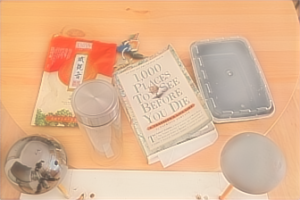
\includegraphics[width=15mm]{images/arch/cari_A1.png}};
    \node[thumb, right=16mm of m.east |- i2] (a2) {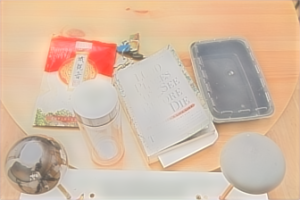
\includegraphics[width=15mm]{images/arch/cari_A2.png}};
    \node[io, above=0.5mm of a1] {$\mathbf{A}_1$}; \node[io, below=0.5mm of a2] {$\mathbf{A}_2$};

    \node[thumb, right=26mm of a1] (s1) {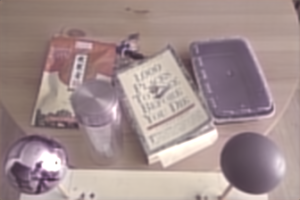
\includegraphics[width=15mm]{images/arch/cari_S1.png}};
    \node[thumb, right=26mm of a2] (s2) {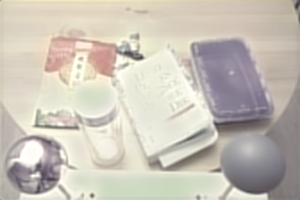
\includegraphics[width=15mm]{images/arch/cari_S2.png}};
    \node[io, above=0.5mm of s1] {$\mathbf{S}_{d,1}$}; \node[io, below=0.5mm of s2] {$\mathbf{S}_{d,2}$};

    % ── flows ──────────────────────────────────────────────────────
    \draw[flow] (i1.east) -- (m.west |- i1);
    \draw[flow] (i2.east) -- (m.west |- i2);
    \draw[flow] (m.east |- a1) -- (a1);
    \draw[flow] (m.east |- a2) -- (a2);
    \draw[flow] (a1.north) to[bend left=18] (s1.north west);
    \draw[flow] (a2.south) to[bend right=18] (s2.south west);

    % ── the two CARI losses ────────────────────────────────────────
    \node[loss] (linv) at ($(a1)!0.5!(a2)$) {$\mathcal{L}_{\text{inv}}$};
    \draw[<->, red!55!black, line width=0.9pt] (a1.south) -- (linv);
    \draw[<->, red!55!black, line width=0.9pt] (a2.north) -- (linv);
    \node[dim, right=0.5mm of linv, text=red!55!black] {$\mathbf{A}_1\!=\!\mathbf{A}_2$\\\scriptsize (material only)};

    \node[loss] (lexp) at ($(s1)!0.5!(s2)$) {$\mathcal{L}_{\text{expl}}$};
    \draw[<->, red!55!black, line width=0.9pt] (s1.south) -- (lexp);
    \draw[<->, red!55!black, line width=0.9pt] (s2.north) -- (lexp);
    \node[dim, right=0.5mm of lexp, text=red!55!black, align=left]
      {$\dfrac{L(\mathbf{S}_{d,1})}{L(\mathbf{S}_{d,2})}\!=\!\dfrac{L(\mathbf{I}_1)}{L(\mathbf{I}_2)}$\\\scriptsize (shading absorbs the cast)};

  \end{tikzpicture}}
  \caption[Cross-Render Albedo Invariance during training.]{%
    Cross-Render Albedo Invariance (CARI), applied only at training time. A pixel-aligned
    pair of the same scene under different coloured illuminants is passed through the
    \emph{same} model (shared weights) in two forward passes. The input thumbnails carry
    visibly different casts, yet the two predicted albedos $\mathbf{A}_1,\mathbf{A}_2$ are
    nearly identical, as enforced by $\mathcal{L}_{\text{inv}}$, while
    the predicted shadings $\mathbf{S}_{d,1},\mathbf{S}_{d,2}$ differ, having absorbed the
    illuminant. $\mathcal{L}_{\text{expl}}$ makes that explicit: it forces the ratio of the
    two shadings to match the ratio of the two inputs, so any colour the albedo declines to
    absorb must be explained by the shading. White balance is disabled for these pairs
    (\secref{sec:raw_pairs}) so that the illuminant colour survives in the input ratio that
    $\mathcal{L}_{\text{expl}}$ reads. Thumbnails are this model's own outputs.
  }
  \label{fig:cari}
\end{figure}

